%Use Lualatex for interpretation!
% lualatex -interaction=nonstopmode --shell-escape UserDocumentation.tex

%You have to have those fonts in your system:
% - Calibri (standard windows font)
% - Trebuchet MS (standard windows font)
% - GROTESKIA (http://www.dafont.com/groteskia.font)

\documentclass[12pt,a4paper]{report}

%\usepackage[utf8]{inputenc} % for old latex interpreters
%\usepackage[english]{babel}

\usepackage{polyglossia}
\setdefaultlanguage[variant=american]{english} % or ?british
\setotherlanguage{czech}

\usepackage{geometry}
\usepackage[cmyk]{xcolor}
\usepackage{amsmath}
\usepackage[some]{background}
\usepackage{listings}
\usepackage{footmisc}
\usepackage{titlesec}
\usepackage{fontspec}
\usepackage{epstopdf,epsfig} 

\definecolor{TextanDarkRed}{cmyk}{.37,.94,.83,.59}
\definecolor{TextanRed}{cmyk}{.0,.879,.844,.220}
\definecolor{javagreen}{rgb}{0.25,0.5,0.35}

\newfontfamily\chapterfont{GROTESKIA}
\newfontfamily\sectionfont{Trebuchet MS}
\titleformat{\chapter}{\chapterfont\fontsize{36pt}{1pt}\selectfont\color{TextanRed}}
  {\thechapter}{20pt}{\chapterfont\fontsize{36pt}{1pt}\selectfont\MakeUppercase}
\titlespacing{\chapter}{0pt}{0pt}{20pt}
\titleformat*{\section}{\LARGE\sectionfont\color{TextanDarkRed}}
\titleformat*{\subsection}{\fontsize{14pt}{1pt}\selectfont\sectionfont\itshape\color{TextanDarkRed}}\titleformat*{\subsubsection}{\sectionfont\color{TextanDarkRed}}

\setmainfont{Calibri}

\backgroundsetup{
scale=1,
angle=0,
opacity=1,
contents={
\begin{tikzpicture}[remember picture,overlay]
  \path [fill=TextanDarkRed] (-0.5\paperwidth,-0.5\paperheight)rectangle (-0.37\paperwidth,0.5\paperheight);
 \end{tikzpicture}}
}

\usepackage[unicode,colorlinks=true]{hyperref}
\hypersetup{pdftitle=TextAn - user documentation}
\hypersetup{pdfauthor={Petr Fanta, Duc Tam Hoang, Adam Huječek, Václav Pernička, Jakub Vlček}}
\hypersetup{linkcolor=black, citecolor=black, urlcolor=black, filecolor=black}

\def\chapwithtoc#1{
\chapter*{#1}
\addcontentsline{toc}{chapter}{#1}
}

% sets numbering for subsubsection
\setcounter{secnumdepth}{3}
\setcounter{tocdepth}{3}

\lstdefinelanguage{properties}{% new language for listings
  basicstyle=\ttfamily,
  sensitive=false,
  morecomment=[l]{\#},      % comment
  morestring=[b]",          % string def
  commentstyle=\color{javagreen},
  basicstyle=\small
}

%Comment macro
%Usage:
% \comment[_assignee_]{_author_}{_comment_}
% \comment{_author_}{_comment_}
\makeatletter
\newcommand{\comment}[3][\@empty]{
  {\color{magenta}[#3 - }
  {\color{green}\ifx\@empty#1\relax Author: #2 \else Assignee: #1; Author: #2\fi}{\color{magenta}]}
}
\makeatother

\newcommand{\textan}{\emph{TextAn}}

\begin{document}

\begin{titlepage}
\BgThispage
\newgeometry{left=4.5cm,top=7cm,bottom=3cm}

\begin{figure}
 
\includegraphics{../CommonImages/TEXTAN_logo_grey_B}
\end{figure}
\noindent
\textcolor{TextanRed}{\chapterfont\fontsize{48pt}{1pt}\selectfont\MakeUppercase{User documentation}}\\[15pt]
\textcolor{TextanDarkRed}{\sectionfont\LARGE\MakeUppercase{Version 0.1}}

\vfill
\noindent
\begin{minipage}[b]{.75\textwidth}
\textbf{Authors}\\
Petr Fanta\\
Duc Tam Hoang\\
Adam Huječek\\
Václav Pernička\\
Jakub Vlček
\end{minipage}% This must go next to `\end{minipage}`
\begin{minipage}[b]{.25\textwidth}
\textbf{Supervisor} \\
Ondřej Bojar\\
%\vfill
\\
\\
\textbf{Date}\\
\today
\end{minipage}

\end{titlepage}
\restoregeometry

\pagenumbering{roman}
\tableofcontents

%\chapter*{Intro}
%\addcontentsline{toc}{chapter}{Intro}


\chapter{User Guide}
\pagenumbering{arabic}

\section{Introduction}

% FOR ENTERTAIN: The spider opens his heavy eyes. He stand up, look through the lousy windows. The sun is flaring, kissing all over the earth. He said to himself: ``It's time''. Students are rushing out of the dormitory like rats desert from a sinking ship. Some are going to the public transport, waiting for the regular hooves from the distance. The bus comes and goes, its double tires sing high notes on the road. Some are visiting the car park. The wheels of the cars creaked around, then they crawled into the city centre. A man and girl are crossing street, with their arms around each other's waists. Then the man must have said something supposed to be funny because two of them are laughing like hyenas. The spider retreats from the windows. The daily screen makes him so lonesome and depressed. Another day has just begun.

%TODO what is textan

%TextAn (Text Analyser) is the product of our software project groups (consists of 5 members) at Faculty of Mathematics and Physics, Charles University in Prague (MFF UK). The tool is attributed to Software Project subject, developed in 9 months from Jan 2014 to Sep 2014, and supervised by RNDr. Ondřej Bojar, PhD. It is a client-server tool which support mining structured information from text documents. At the moment, the documents are specified to police report but TextAn could be applied to a wide range of domains. 

% --> to DeveloperDocumentation
% 

%TODO basic usage


\subsection{System overview}

%What is this?

%what textan do, something which is 

%WHAT DOES THE POLICE WANT? OF COURSE NOT ARREST US

% 

% it should be something better, for example, what textan to in a : What textan to. what you can expect in the rest of documentation . If you don't need what we offer in textan, leave a comment and get away.



With the profiliferation of unstructured written texts, the need for a tool to mine the structure out of such documents is on increasing trend. 
\textan{} (Text Analyser) serves such purpose, targeting the Police's reports. 
In other words, \textan{} is a tool which supports mining structured data buried in the Police's reports. The term ``structured data'' consists of two concepts. 
First, it contains name, street, date of birth, crime and other named entities with related to some people. 
Second, the data contain the relations between two entities. 
For example, the relation between a person and his/her name, the relation between two persons. The objective of \textan{} is to provide a robust tool which support the procedure, either automatically and manually.

\textan{} has client-server structure. It supports following operations:
  
  \begin{itemize}
  \item Bring new solution to the classic problem of extracting data from text.
  \item Provide the service for both automatic detection and manual adjustment.
  \item Make the adjustment of data as simple as possible for users.
  \item Make the graphic user interface as fruitful as possible.
  \end{itemize}

This documentation describes \textan{} from the perspective of an user. 
All the concepts are explained in the \emph{Glossary}.

To start using \textan{}, user have to start the client application and log in. 
Once user log in successfully, the main screen of \textan{} is displayed.

\comment{Tam}{What's next?} 

\subsection{Glossary}

\comment{Petr}{definitions of terms in documentation and applications}

\subsection{Conventions}
\comment{Petr}{is this section needed?}

\section{Client Usage}

This section contains all information needed by end users to sucessfully use
the \textan{} client application. For instructions to actual run the client
see \ref{sssec:StartClient}.

\subsection{First Run}

On the first \textan{} client run users are promted to enter their username
(see figure \ref{fig:Login}, which is used by the system to identify the users.
The login name is stored in settings and the login dialog is not shown again
next runs. It can be changed later in settings (see \ref{ssec:Settings}). The
valid name is required, ie. not empty and not whitespace characters only. If
users enter invalid login, a warning is displayed and they can enter other
login or the application quits.

\begin{figure}[!htb]
        \centering
        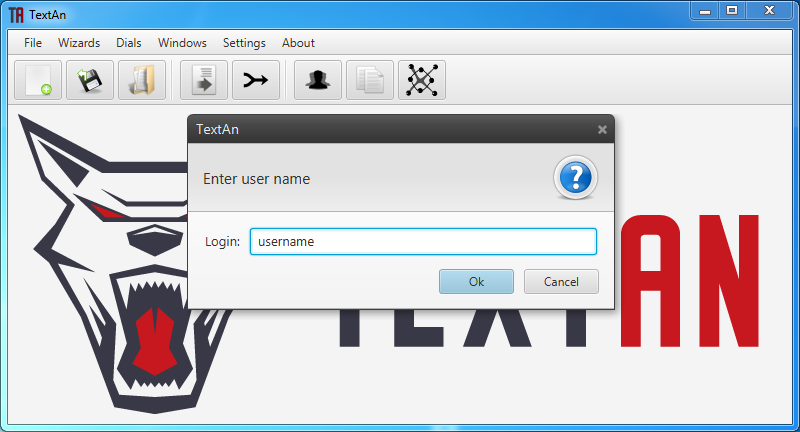
\includegraphics[width=\textwidth]{Images/login}
        \caption{Login prompt on first run.}
        \label{fig:Login}
\end{figure}

\subsection{Working Space}

The \textan{} client's application working space is very simple and intuitive.
The main window (see figure \ref{fig:MainWindow}) contains main menu bar with
all commands needed to control the application. The individual items are sorted
out into categories to make the orientation easier. There is also toolbar with
icons for mostly used commands to speed up the access to them.

\begin{figure}[!htb]
        \centering
        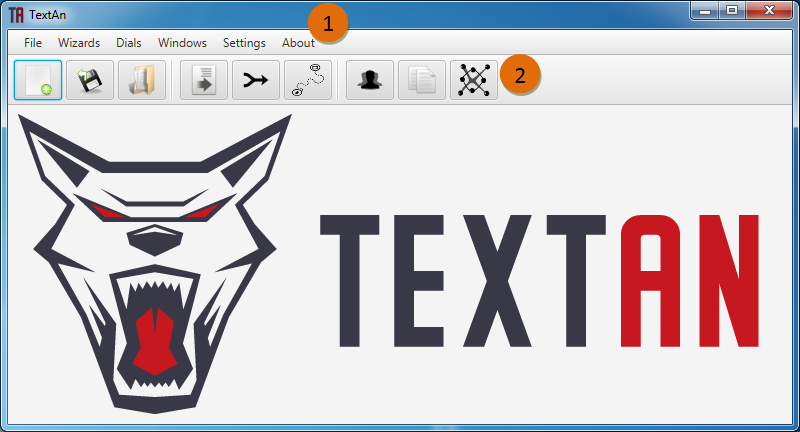
\includegraphics[width=\textwidth]{Images/main}
        \caption{Main window controls.}
        \label{fig:MainWindow}
\end{figure}

The File menu contains items to create new report, import report from external
file and load report whose processing was not finished, but saved to continue
later. For more information about report processing see \ref{ssec:ProcessReport}.

The Wizards menu contains items starting wizards to guide the users in more
complicated tasks, like processing report (see \ref{ssec:ProcessReport}) and
joining objects (see \ref{ssec:JoinObjects}).

The Dials menu contains items to display objects, documents and relations
stored in the database (see \ref{ssec:ViewDatabase}).

The Windows menu contains the list of currently displayed application windows
to easily bring the windows to front.

The Settings menu contains items to customize \textan{} client appearance and
behaviour. For more information see \ref{ssec:Settings}. It also contains
shortcut to reset the position and size of the main window.

\subsection{Settings}
\label{ssec:Settings}

This section describes options available in individual items contained in the
main menu Settings.

\subsection{General Settings}
\label{sssec:GeneralSettings}

The General Settings window (see figure \ref{fig:GeneralSettings}) contains
controls for changing the behaviour and appearance of the application.

\begin{figure}[!htb]
        \centering
        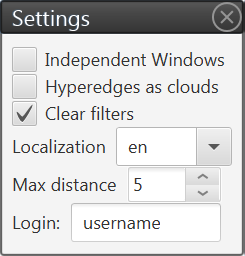
\includegraphics[width=\textwidth]{Images/general}
        \caption{General Settings Window}
        \label{fig:GeneralSettings}
\end{figure}

\paragraph{Independent Windows} If this control is checked the application
secondary windows will not be embedded into the main window, but separate
independent system windows will be used.

\paragraph{Hypergraphs} This control affects the rendering of hyperedges%
\footnote{Hyperedge is an edge in a hypergraph. It is a generalization of
term graph. The difference is that edges in hypergraphs can connect any number
of nodes, but in graph they always connect two nodes.}
in graphs (see figure \ref{fig:Hypergraphs}). The default rendering transforms
hypergraphs to graphs by adding auxiliary nodes of square shape representing
the relation. If this control is checked, the edges are rendered by graph
background.

\begin{figure}[!htb]
        \centering
        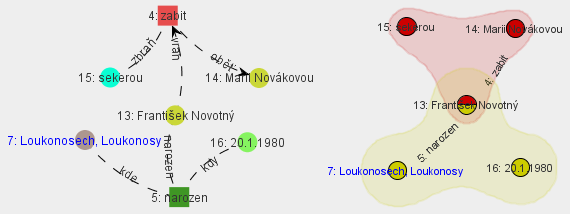
\includegraphics[width=\textwidth]{Images/hypergraphs}
        \caption{Graph rendering differences. Default on the left.}
        \label{fig:Hypergraphs}
\end{figure}

\paragraph{Clear Filters} If this control is checked the filter fields
displayed during report processing will be cleared when shown again.

\paragraph{Localization} This control determines the language of the \textan{}
client. The Czech and English localizations are currently supported. The
default language is English. Changing localization takes effect after
restarting the application.

\paragraph{Graph Distance} This control affects default maximal length of the
path between any node and the graph central node.

\paragraph{Login} This control enables users to change their username. Changing
login takes effect after restarting the application.

\subsection{Report Processing}
\label{ssec:ProcessReport}

Wizard for report processing is accessible from the main menu. It guides
users in complicated procedure of processing a report. The procedure is divided
into several steps described in this section. Users can return to previous
steps, but if any changes are done, the progress in following steps are lost.

\subsubsection{Report Source}

\begin{figure}[!htb]
        \centering
        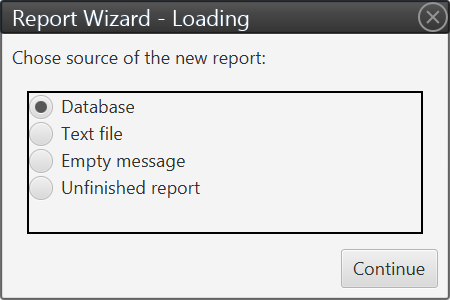
\includegraphics[width=\textwidth]{Images/source}
        \caption{Choosing report source.}
        \label{fig:Source}
\end{figure}

This step (see figure \ref{fig:Source} allows users to chose the source of the
report. There are following sources:

\paragraph{Database} This option displays (see figure \ref{fig:Database}) list
of all unprocessed reports stored in the database (for filtering details see
\ref{sssec:DocumentList}).
The report cannot be edited, so the wizard then proceeds to Edit Entities step (see \ref{sssec:EditEntities}).

\begin{figure}[!htb]
        \centering
        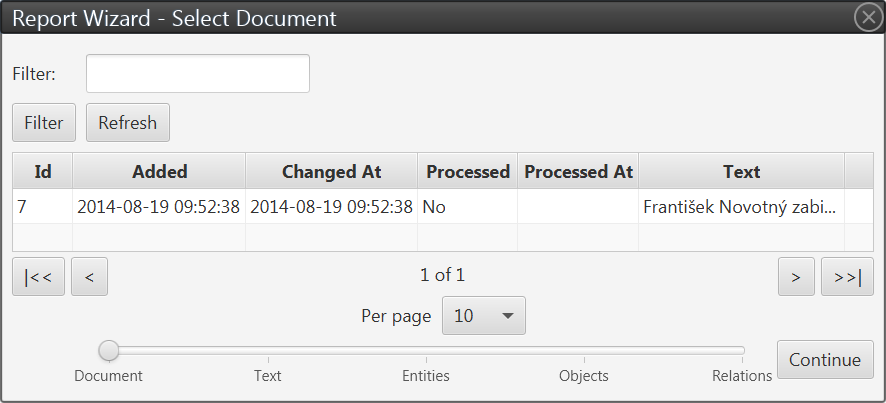
\includegraphics[width=\textwidth]{Images/database}
        \caption{Chosing report from database.}
        \label{fig:Database}
\end{figure}

\paragraph{Text File} This option displays open file dialog for importing
report text from external file. The extracted text is then displayed (see
figure \ref{fig:TextFile}, so users can chose the proper file encoding. Then
the wizard proceeds to Report Edit step (see \ref{sssec:ReportEdit}).

\begin{figure}[!htb]
        \centering
        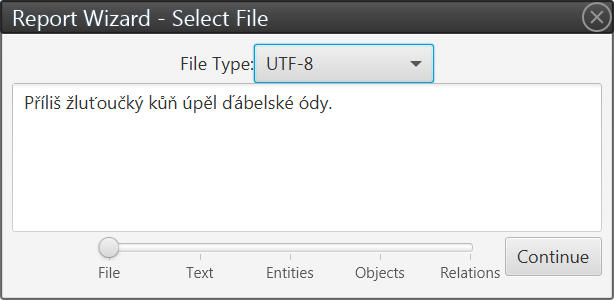
\includegraphics[width=\textwidth]{Images/textfile}
        \caption{Chosing encoding of the file.}
        \label{fig:TextFile}
\end{figure}

\paragraph{Empty Message} This option proceeds directly to Report Edit step
(see \ref{sssec:ReportEdit}).

\paragraph{Unfinished Report} This option displays open file dialog for
selecting the file with report whose processing has not been finished, but it
was stored to continue later. The wizards then proceeds to step where report
processing has been interupted.

\subsubsection{Edit Report}
\label{sssec:ReportEdit}

In this step users can edit the text of the report (see figure
\ref{fig:ReportEdit}. This step is followed by Edit Entities step (see
\ref{sssec:EditEntities}).

\begin{figure}[!htb]
        \centering
        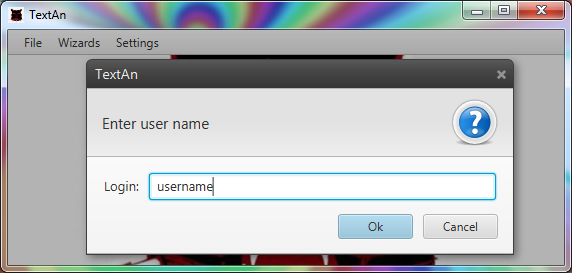
\includegraphics[width=\textwidth]{Images/reportedit}
        \caption{Editing the text of the report.}
        \label{fig:ReportEdit}
\end{figure}

\subsubsection{Edit Entities}
\label{sssec:EditEntities}

Before entering this step the system automatically recognizes named entities
in the report text. Recognized entities are marked by text color. Entities of
the same type has the same color (see \ref{fig:Entities}). Hovering over entity
text will display its type.

Users can correct recognized entities and add new ones by selecting the text
of the entity by mouse and picking the entity type from the context menu.
There is a filter field in the context menu to allow users enter part of name
of the desired entity type to speed up the selection process. If there are only
one item in the list left, it can be selected by pressing enter too. Pressing
Down key in the filter field transfers focus to the list, so keybord keys Up,
Down and Enter can be used to select the entity type.

One entity cannot comprise from several separated parts and entities cannot
overlapped.

This step is followed by Edit Objects step (see \ref{sssec:EditObjects}).

\begin{figure}[!htb]
        \centering
        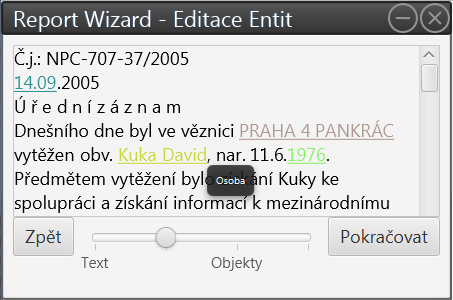
\includegraphics[width=\textwidth]{Images/entities}
        \caption{Editing entities in the report.}
        \label{fig:Entities}
\end{figure}

\subsubsection{Edit Objects}
\label{sssec:EditObjects}

In this step the entities are assigned to real objects (see figure
\ref{fig:Objects}. The system automatically assigns objects stored in the
database to entities recognized in the database. If no suitable object is
found, the entity is marked with orange background. Hovering over entity
displays its type and assigned object if any.

\begin{figure}[!htb]
        \centering
        
\includegraphics[width=\textwidth]{Images/objects}
        \caption{Editing objects in the report.}
        \label{fig:Objects}
\end{figure}

Right click on objects will display context menu with options to show the graph
of the object or documents containing the object. This is also true for all following steps.

To assign object to entity left click the entity and select suitable object
from the context menu (see \ref{fig:ObjectMenu}) or create entirely new object.

\begin{figure}[!htb]
        \centering
        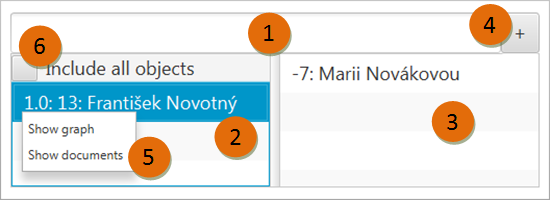
\includegraphics[width=\textwidth]{Images/objectmenu}
        \caption{Menu for selecting object. 1) Filter field, 2) List of recommended objects, if 6) is checked, list of objects of given type from database, 3) List of new objects created during editation of the same type, 4) Button for creating new object, 5) Menu for more information about the object.}
        \label{fig:ObjectMenu}
\end{figure}


The report processing cannot continue unless all entities have assigned
objects. This step is then followed by Relation Edit step (see
\ref{sssec:EditRelations}).

\subsubsection{Edit Relations}
\label{sssec:EditRelations}

This is the last mandatory step during report processing (see figure
\ref{fig:Relations}). It consist of marking relationships between objects in
the document. There are two types of relations: with anchor%
\footnote{Anchor is a word or phrase determining the relation, typically
sentence predicate.}
and without anchor.

\begin{figure}[!htb]
        \centering
        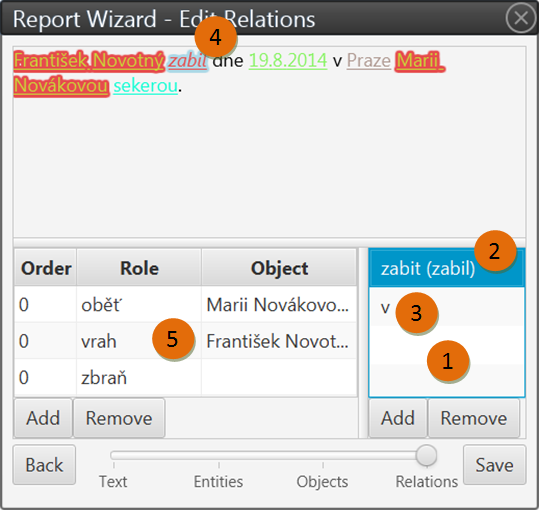
\includegraphics[width=\textwidth]{Images/relations}
        \caption{Editing relations in the report.}
        \label{fig:Relations}
\end{figure}

Relation with anchor can be created by selecting the words of the anchor by
mouse and picking a relation type from context menu. Empty relation with given
anchor and type is added to the list of relations. Empty relation without anchor
can be added by Add button under the relation list. New relations will have
prefilled some roles based on relations of that type already stored in the
database. Selecting relation will highlight its anchor and assigned objects.

To add an object to a relation, select the relation in the list of relations.
Use Add button under object list to add new row to the object table. Double
clicking the object cell opens combobox with the list of objects in the report
to assign to the relation. Or you can drag the object from the report text and
drop it to empty row or Add button to add new row. Dropping the object into the
non empty row replaces the assigned object.

After finishing relation editation the document is stored to the database,
unless some errors occur. In that case Error Step follows (see
\ref{sssec:Errors}).

\subsubsection{Errors}
\label{sssec:Errors}

This step takes place only if some changes to the database from other sources
are detected (see figure \ref{fig:Errors}). The window informs user which new
objects and relations have been created while the report was being processed and
which objects have been joined. Users can decide to return to previous steps
and reconsider their edits or force the saving of the report.

\begin{figure}[!htb]
        \centering
        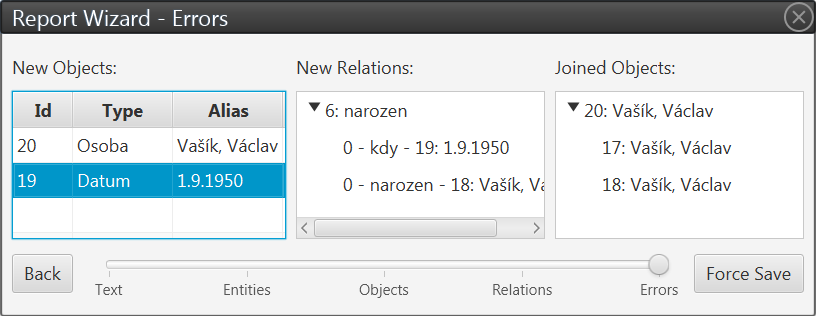
\includegraphics[width=\textwidth]{Images/errors}
        \caption{Errors when saving report.}
        \label{fig:Errors}
\end{figure}

\subsection{View Database}
\label{ssec:ViewDatabase}

Users can use client to view data stored in the database by selecting items
in Dials menu of the main window. Other ways include various context menus
while processing reports etc.

\subsubsection{View Objects}
\label{sssec:ObjectList}

This window contains list of objects matching the filter criteria (alias text,
object type) paginated for more convenient work (see figure \ref{fig:ObjectList}.
Please note that changing filter criteria must be confirmed by pressing Filter
button. Use right mouse button click to open context menu for displaying graph
for the selected object (see \ref{ssec:Graphs}) or for displaying list of documents containing it (see \ref{sssec:DocumentList}).

\begin{figure}[!htb]
        \centering
        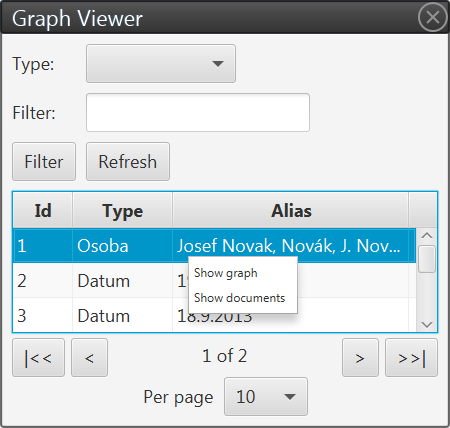
\includegraphics[width=\textwidth]{Images/objectlist}
        \caption{List of objects.}
        \label{fig:ObjectList}
\end{figure}

\subsubsection{View Documents}
\label{sssec:DocumentList}

This window contains list of documents matching filter criteria. Please note
that not all filter controls may be visible at all situations as they are
customized to fit the current context (see figure \ref{fig:DocumentList}.
Please note that changing filter criteria must be confirmed by pressing Filter
button. Use right mouse button click to open context menu for displaying graph
for the selected document (see \ref{ssec:Graphs}) or for displaying the report
itself (see \ref{sssec:DocumentView}). Other options include editing the report
or processing it if possible. Hovering over the row displays full report text.

\begin{figure}[!htb]
        \centering
        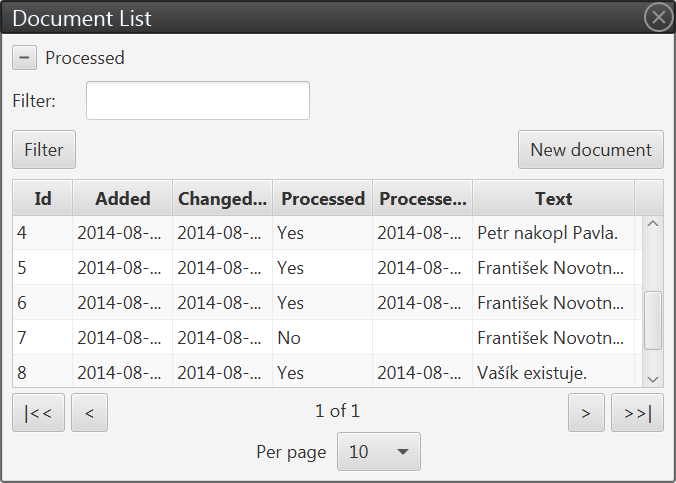
\includegraphics[width=\textwidth]{Images/documentlist}
        \caption{List of documents.}
        \label{fig:DocumentList}
\end{figure}

\subsubsection{View Document}
\label{sssec:DocumentView}

This window displays reports with highlighted objects and relations for easier
orientation (see \ref{fig:DocumentView}). Use right mouse click to open object
context menu to get more information about the selected object. Selecting
relation will highlight its anchor and assigned objects.

\begin{figure}[!htb]
        \centering
        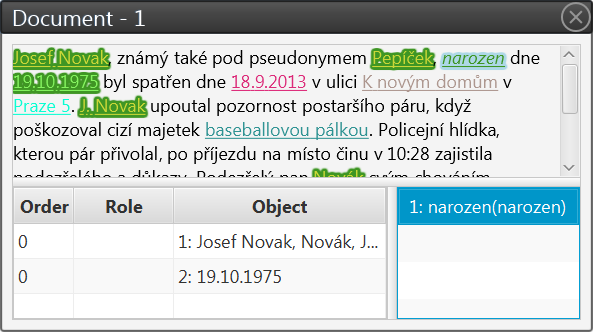
\includegraphics[width=\textwidth]{Images/documentview}
        \caption{Document detail.}
        \label{fig:DocumentView}
\end{figure}

\subsubsection{View Relations}

This window contains list of relations matching the filter criteria (anchor
text, relation type) paginated for more convenient work (see figure
\ref{fig:RelationList}. Please note that changing filter criteria must be
confirmed by pressing Filter button. Use right mouse button click to open
context menu for displaying graph for the selected relation (see \ref{ssec:Graphs})
or for displaying list of documents containing it (see \ref{sssec:DocumentList}).

\begin{figure}[!htb]
        \centering
        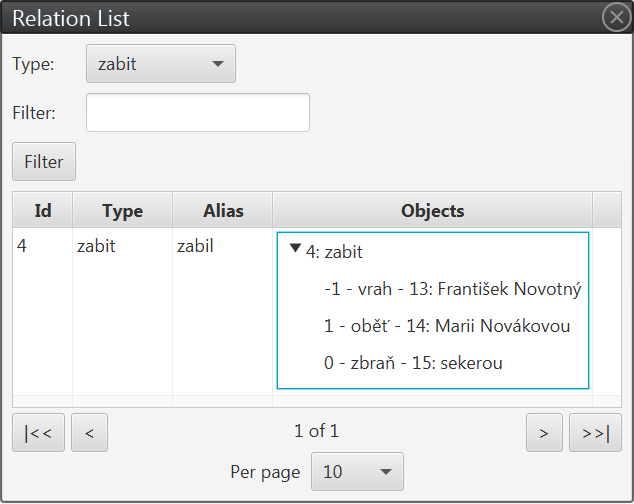
\includegraphics[width=\textwidth]{Images/relationlist}
        \caption{List of relations.}
        \label{fig:RelationList}
\end{figure}

\subsection{Graph Views}
\label{ssec:Graphs}

Graph Windows can be displayed from many places in \textan{} client. Most
common way is right clicking an object/relation/document and selecting Show
graph context menu item.

The graph appearance is drastically effected by Hypergraphs settings (see
\ref{sssec:GeneralSettings}).

In the top part of the window (see figure \ref{fig:Graph}) there is a toolbar
with icons to manipulate the graph.

The first icon represents Transformation and is used to manipulate the graph as a whole, eg. panning or rotating (hold CTRL while left clicking and moving the
mouse). The second icon represents Picking and is used to manipulate subset of nodes. Hold left mouse button and drag to select multiple nodes and then click and drag to move them. Distance field can be used to change the "radius" around the central node. Use mousewheel to zoom the graph.

Nodes representing objects can be right clicked to show context menu with
options to display their surroundings or documents. Right clicking edges or
nodes representing the relations shows context menu for centering to objects
assigned to the relation.

On the sides there are lists of object/relation types to display. Unchecking
the type will cause objects/relations of that type to disappear when graph is refreshed by Go button. Clicking the three dots will show or hide the filter
lists.

\begin{figure}[!htb]
        \centering
        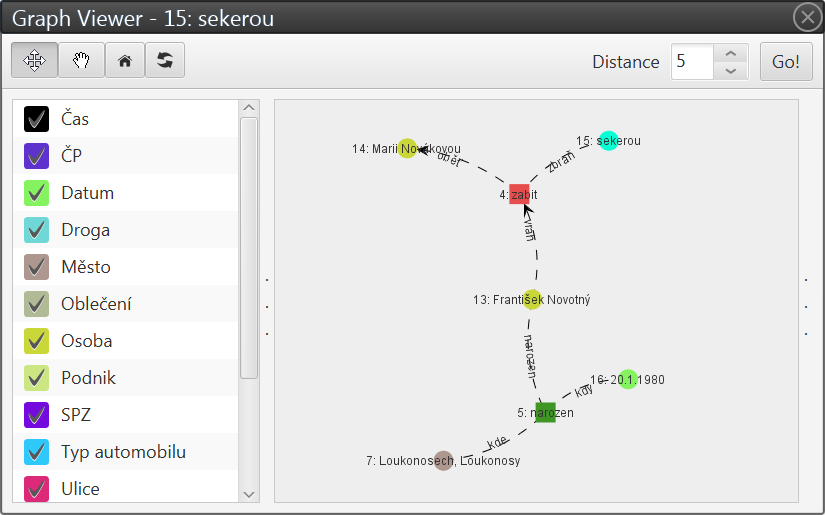
\includegraphics[width=\textwidth]{Images/graph}
        \caption{Graph window.}
        \label{fig:Graph}
\end{figure}

\subsection{Joining Objects}
\label{ssec:JoinObjects}

There can be situations when it is discovered that two objects originaly
thought to be independent are in fact one object. For such cases there is Join
Object wizard (see figure \ref{fig:Join}). For more information about object
lists see \ref{sssec:ObjectList}.

\begin{figure}[!htb]
        \centering
        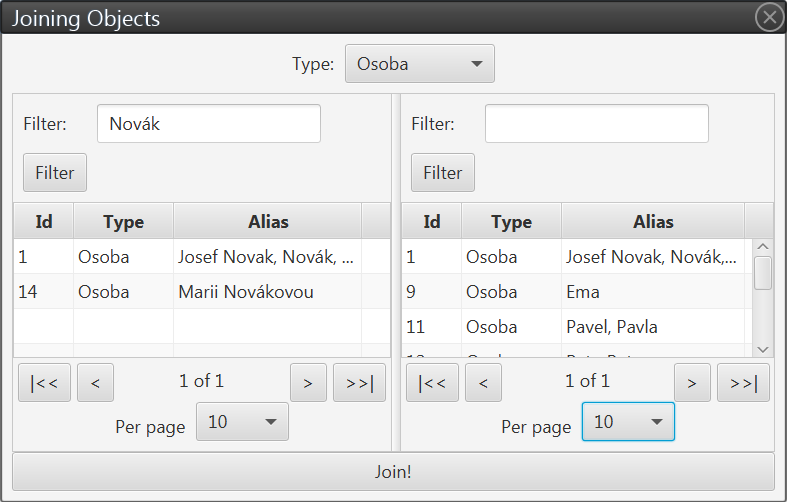
\includegraphics[width=\textwidth]{Images/join}
        \caption{Join Object Wizard.}
        \label{fig:Join}
\end{figure}

The objects to merge must have common type. Select one object in left object
list and the other one in right object list. The button Join will start the
joining itself.

\chapter{Administrator guide}

\section{Server}

\subsection{Installation guide}


This section will show you how to install and build \textan{} server. 
%An installation guide for a server side application of \textan{}.

\subsubsection{Prerequisites}
\label{sssec:SerInstPre}

The \textan{} server requires installation of \emph{Java 8 JRE%
\footnote{We recommend to use JRE from \emph{Oracle}, available at: \url{http://www.oracle.com/technetwork/java/javase/downloads/index.html}}}
or a later version and a relational database system (e.g. \emph{MySQL}).
The server should be platform independent, so it runs on any system where JRE is available,
but it depends on native and 3rd party libraries. 
Supported operating systems in the distribution of the \textan{} server are
Linux (32 bit and 64 bit) and Windows (32 bit and 64 bit). \comment[Petr]{Petr}{Finish this...}

\subsubsection{Installation}

The \textan{} server distribution archive contains all files needed for \textan{} server to operate,
such as server binaries, native libraries, run scripts and additional resources.
For installation it is sufficient to unpack its content into any directory.

\subsubsection{Basic configuration}

Before the first start, it is necessary to set up the server and the database.

\comment[Petr,Jakub,Venca]{Petr}{write how to setup server}

\comment[Petr]{Petr}{add some link to \ref{sec:ServerSettings}}

\subsubsection{Starting the server}

The server can be started by starting scripts in its root directory. 
Scripts for different operating systems unfortunately do not provide the same functionality.

The start script for the Linux-based operating system (\emph{run.sh}) runs the server application as daemon
and can be used to run the server as system service.

The start script for the Microsoft Windows OS is less powerful, only runs the server application. 
To run the server as a background process, the Windows Service is required. 
Unfortunately, there are no components shipped with the Jetty Distribution to make it a formal Windows Service.
However, we recommend the use of \emph{Apache ProcRun's Daemon%
\footnote{More information can be found on \url{https://commons.apache.org/proper/commons-daemon/procrun.html} and in JavaDoc documentation for \emph{cz.cuni.mff.ufal.textan.server.AppEntry} class.}}.

\subsection{Settings}
\label{sec:ServerSettings}

\subsubsection{Web server settings}

%connector
\paragraph{server.connector.host} The particular interface to listen on. If not set or 0.0.0.0, the web server listens on port on all interfaces.

\paragraph{server.connector.port} The port to listen on. If not set, the web server listens on port 9500.

%thread pool
\paragraph{server.threadPool.maxThreads} The maximum number of threads in web server thread pool. It determines a maximum number of simultaneously opened connections. The default value is 200.

\paragraph{server.threadPool.minThreads} The minimum number of threads in web server thread pool. The default value is 8.

\paragraph{server.threadPool.idleTimeout} The time in milliseconds that the connection can be idle before it is closed.

%ssl
\paragraph{server.ssl}
\paragraph{server.ssl.keyStore.path}
\paragraph{server.ssl.keyStore.password}
\paragraph{server.ssl.keyManager.password}
\paragraph{server.ssl.keyStore.type}
\paragraph{server.ssl.port}

%ssl client auth
\paragraph{server.ssl.clientAuth}
\paragraph{server.ssl.trustStore.path}
\paragraph{server.ssl.trustStore.password}
\paragraph{server.ssl.trustStore.type}

\subsubsection{Database connection settings}
\comment[Venca]{Petr}{Add descrtion for DB properties}
%jdbc
\paragraph{jdbc.driverClassName}
Name of the driver class made usually by database developers which enables to interact with database.

\paragraph{jdbc.url}
 The url that points to our database. The most common url format is like this:
jdbc:[database type]:[hostname]:[port number]/[database name]
and is specific to the driver we use.

\paragraph{jdbc.user}
Username to log into the database.
\paragraph{jdbc.pass}
Password to authorize the user in database.

%c3p0 (http://www.mchange.com/projects/c3p0/#configuration_properties)
\paragraph{c3p0.maxPoolSize}
Maximum number of Connections a pool will maintain at any given time.

\paragraph{c3p0.minPoolSize}
Minimum number of Connections a pool will maintain at any given time.

\paragraph{c3p0.initialPoolSize}
Number of Connections a pool will try to acquire upon startup. Should be between minPoolSize and maxPoolSize.

\paragraph{c3p0.acquireIncrement}
Determines how many connections at a time c3p0 will try to acquire when the pool is exhausted.

\paragraph{c3p0.maxIdleTime}
Seconds a Connection can remain pooled but unused before being discarded. Zero means idle connections never expire.

\paragraph{c3p0.checkoutTimeout}
The number of milliseconds a client calling getConnection() will wait for a Connection to be checked-in or acquired when the pool is exhausted. Zero means wait indefinitely. Setting any positive value will cause the getConnection() call to time-out and break with an SQLException after the specified number of milliseconds.

\paragraph{c3p0.maxStatements}
The size of c3p0's global PreparedStatement cache. If both maxStatements and maxStatementsPerConnection are zero, statement caching will not be enabled. If maxStatements is zero but maxStatementsPerConnection is a non-zero value, statement caching will be enabled, but no global limit will be enforced, only the per-connection maximum. maxStatements controls the total number of Statements cached, for all Connections. If set, it should be a fairly large number, as each pooled Connection requires its own, distinct flock of cached statements. As a guide, consider how many distinct PreparedStatements are used frequently in your application, and multiply that number by maxPoolSize to arrive at an appropriate value. Though maxStatements is the JDBC standard parameter for controlling statement caching, users may find c3p0's alternative maxStatementsPerConnection more intuitive to use. 

\paragraph{c3p0.maxStatementsPerConnection}
The number of PreparedStatements c3p0 will cache for a single pooled Connection. If both maxStatements and maxStatementsPerConnection are zero, statement caching will not be enabled. If maxStatementsPerConnection is zero but maxStatements is a non-zero value, statement caching will be enabled, and a global limit enforced, but otherwise no limit will be set on the number of cached statements for a single Connection. If set, maxStatementsPerConnection should be set to about the number distinct PreparedStatements that are used frequently in your application, plus two or three extra so infrequently statements don't force the more common cached statements to be culled. Though maxStatements is the JDBC standard parameter for controlling statement caching, users may find maxStatementsPerConnection more intuitive to use.

\paragraph{c3p0.idleConnectionTestPeriod}
If this is a number greater than 0, c3p0 will test all idle, pooled but unchecked-out connections, every this number of seconds.

%hibernate
\paragraph{hibernate.dialect}
The classname of a Hibernate org.hibernate.dialect.Dialect which allows to generate SQL optimized for a particular relational database.
\paragraph{hibernate.show\_sql}
If true all sql statements are written to console. It's an alternative for logging.

%NameTag
\subsubsection{Named entity recognizer settings}
This section is mainly about settings stored in NametagLearning.properties.
There are parameters for neural network which nametag use for learning and switches for nametag functions.
Also, there are settings for affecting models storing and learning data generating.
All inputs are assumed to be in UTF-8 encoding.


\paragraph{ner\_identifier}
Identifier of the named entity recognizer type. This affects the tokenizer used in this model, and in theory any other aspect of the recognizer. Supported values are:
\begin{description}
\item[$\cdot$] czech
\item[$\cdot$] english
\item[$\cdot$] generic
\end{description}

\paragraph{tagger}
Identifier of tagger. NameTag can utilize several taggers to obtain the tags and lemmas:

\begin{description}
\item[$\cdot$ trivial] Do not use any tagger. The lemma is the same as the given form and there is no part of speech tag.
\item[$\cdot$ external] Use some external tagger. The input "forms" can contain multiple tab-separated values, first being the form, second the lemma and the rest is part of speech tag. The part of speech tag is optional. The lemma is also optional and if missing, the form itself is used as a lemma.
\item[$\cdot$ morphodita:model] Use MorphoDiTa as a tagger with the specified model. This tagger model is embedded in resulting named entity recognizer model. The lemmatizer model of MorphoDiTa is recommended, because it is very fast, small and detailed part of speech tags do not improve the performance of the named entity recognizer significantly.
\end{description}

\paragraph{featuresFile}
Path of generated file, based on property file 
The recognizer utilizes feature templates to generate features which are used as the input to the named entity classifier. The feature templates are specified in a file, one feature template on a line. Empty lines and lines starting with \# are ignored.

The first space-separated column on a line is the name of the feature template, optionally followed by a slash and a window size. The window size specifies how many adjacent words can observe the feature template value of a given word, with default value of 0 denoting only the word in question.

List of commonly used feature templates follows. Note that it is probably not exhaustive (see the sources in the features directory).

\paragraph{stages}
The number of stages performed during recognition. Common values are either 1 or 2. With more stages, the model is larger and recognition is slower, but more accurate.

\paragraph{iterations}
The number of iterations performed when training each stage of the recognizer. With more iterations, training take longer (the recognition time is unaffected), but the model gets over-trained when too many iterations are used. Values from 10 to 30 or 50 are commonly used.

\paragraph{missing\_weight}
Default value of missing weights in the log-linear model. Common values are small negative real numbers like -0.2.

\paragraph{initial\_learning\_rage}
learning rate used in the first iteration of SGD training method of the log-linear model. Common value is 0.1.

\paragraph{final\_learning\_rage}
learning rate used in the last iteration of SGD training method of the log-linear model. Common values are in range from 0.1 to 0.001, with 0.01 working reasonably well.

\paragraph{gaussian}
The value of Gaussian prior imposed on the weights. In other words, value of L2-norm regularizer. Common value is either 0 for no regularization, or small real number like 0.5.

\paragraph{hidden\_layer}
Experimental support for hidden layer in the artificial neural network classifier. To not use the hidden layer (recommended), use 0. Otherwise, specify the number of neurons in the hidden layer. Please note that non-zero values will create enormous models, slower recognition and are not guaranteed to create models with better accuracy.

\paragraph{heldout\_data}
Optional parameter with heldout data in the described format. If the heldout data is present, the accuracy of the heldout data classification is printed during training. The heldout data is not used in any other way.

\paragraph{waiting\_time}
Maximum time for learning new model (only when learning is blocking - model doesn't exist)

\paragraph{default\_training\_data\_file}
Sample file with initial training data, which is copied before training data generated from database. When this property is empty, no default training data are used.

\paragraph{maximum\_stored\_models}
Number of maximum stored models. When limit is exceeded, the oldest models are deleted

\paragraph{form}
Size of window when forms are used as features (0 when are not used)

\paragraph{lemma}
Size of window when lemma ids are used as features (0 when are not used)

\paragraph{raw\_lemma}
Size of window when raw lemmas are used as features (0 when are not used)

\paragraph{raw\_lemma\_capitalization}
Size of window when capitalization of raw lemma is used as features (0 when are not used)

\paragraph{tag}
Size of window when tags are used as features (0 when are not used)

\paragraph{numeric\_time\_value}
recognize numbers which could represent hours, minutes, hour:minute time, days, months or years

\paragraph{czech\_lemma\_term}
feature template specific for Czech morphological system by Jan Hajič (Hajič 2004). The term information (personal name, geographic name, ...) specified in lemma comment are used as features.

\paragraph{brown\_clusters}size of window foe Brown clusters 

\paragraph{brown\_clusters\_file}
Use Brown clusters found in the specified file. An optional list of lengths of cluster prefixes to be used in addition to the full Brown cluster can be specified. Each line of the Brown clusters file must contain two tab-separated columns, the first of which is the Brown cluster label and the second is a raw lemma.

\paragraph{gazetteers}
Size of window when gazetteers are used (0 when are not used)

\paragraph{gazetteers\_directory}
Directory of gazetteers files. Each file is one gazetteers list independent of the others and must contain a set of lemma sequences, each on a line, represented as raw lemmas separated by spaces.

\paragraph{previous\_stage}
use named entities predicted by previous stage as features

\paragraph{email\_detector}
Detect URLs and emails. If an URL or an email is detected, it is immediately marked with specified named entity type and not used in further processing.

\subsection{Data formats}

\section{Client}

This section contains all information needed to successfully install, configure
and run \textan{} JavaFX client side application. However thanks to \textan{}
client-server architecture and extensive use of webservices, it is easy to
prepare own implementation in any programmer language desired or even use
general solutions as SoapUI%
\footnote{More information can be found at \url{http://www.soapui.org/}},
if \textan{} default client does not provide all required features, user
experience or integration to legacy system is needed.

\subsection{Installation guide}

This section describes how to install and configure \textan{} client on
workstations of end users.

\subsubsection{Prerequisites}

The \textan{} client has the same requirement for \emph{Java 8 JRE} or later
as the server (see \ref{sssec:SerInstPre}). However, unlike the server side,
it is pure Java application so there are no other additional limitations for
operating system etc. Any platform where JRE 8 is available can support the
client.

\subsubsection{Installation}

Unpack an archive with the \textan{} client distribution into any directory. 
The archive contains a .jar file and starting scripts for the
\emph{Microsoft Windows} and Linux-based operating systems%
\footnote{run.bat for MS Windows and run.sh for Linux clones.\label{runscript_note}}.

\subsubsection{Basic configuration}

If the client is not supposed to connect to the default server, it is necessary
to configure a server location. The client settings are by default stored in \emph{TextAn.properties\footnote{A description of format of .properties file can be found at \url{http://en.wikipedia.org/wiki/.properties}}}
in the client directory. Simply edit or add following lines to properties file
(create it if it does not exist), replacing default server address with the
actual one:
\begin{lstlisting}[frame=single,language=properties]
#url of the document processor
url.document=http://localhost:9500/soap/document
#url of the document processor wsdl
url.document.wsdl=http://localhost:9500/soap/document?wsdl
#url of the data provider
url.data=http://localhost:9500/soap/data
#url of the data provider wsdl
url.data.wsdl=http://localhost:9500/soap/data?wsdl
\end{lstlisting}

If SSL is in use, it needs to be configured by setting following properties:
\begin{lstlisting}[frame=single,language=properties]
#should ssl be used for communication?
ssl=true
#path to trust store
ssl.trustStore=c\:/temp/clientTrustStore
#trust store password
ssl.trustStore.password=MYPASS
#trust store type
ssl.trustStore.type=JKS
\end{lstlisting}

If client authorization is in use along with SSL, it needs to be configured
by settings following properties:
\begin{lstlisting}[frame=single,language=properties]
#should client authorization be used for communication?
ssl.clientAuth=true
#path to key store
ssl.keyStore=c\:/temp/clientKeyStore
#key store password
ssl.keyStore.password=MYPASS
#key store type
ssl.keyStore.type=JKS
\end{lstlisting}

\subsubsection{Starting the client}
\label{sssec:StartClient}

The .jar file from the distribution archive is executable,
but we recommend to use starting scripts\footref{runscript_note}.
Please consult documentation of your Java Platform provider,
if running scripts are not available for your system.
For description of command line arguments see \ref{ssec:CliCmdArg}

\subsubsection{Uninstallation}

The client application does not use any files or resources outside its install
directory, unless explicitly told to do otherwise.
To uninstall the client just delete its installation folder and all files
explicitly used as configuration storage.

\subsection{Settings}

This section describes all settings affecting the client behaviour.
The two basic means are command line arguments and configuration file in
properties format.

\subsubsection{Command line arguments}
\label{ssec:CliCmdArg}

The client has one command line option (-h, --help, /H, /?) which displays the
usage information. Apart from that it takes only one command line argument
which is the location of settings file. If no file is specified, default
property file \emph{TextAn.properties} will be used. If '-' is provided, the
standard input will be read and settings will not be stored.

\subsubsection{TextAn.properties}

For complete list of properties stored in TextAn.properties, please see
Developer Documentation apendix Client Properties in TextAn.properties.

\comment[latex expert, Peter?]{Adam}{Please, someone more skilled in latex use
proper way to reference the other document. Thanks.}

For more information about \emph{clear.filters}, \emph{graph.distance},
\emph{hypergraphs}, \emph{locale.language}, \emph{username}
and \emph{windows.independent} please see \ref{sssec:GeneralSettings}.

\end{document}
